\documentclass[11pt]{article}\usepackage[]{graphicx}\usepackage[]{color}
%% maxwidth is the original width if it is less than linewidth
%% otherwise use linewidth (to make sure the graphics do not exceed the margin)
\makeatletter
\def\maxwidth{ %
  \ifdim\Gin@nat@width>\linewidth
    \linewidth
  \else
    \Gin@nat@width
  \fi
}
\makeatother

\definecolor{fgcolor}{rgb}{0.345, 0.345, 0.345}
\newcommand{\hlnum}[1]{\textcolor[rgb]{0.686,0.059,0.569}{#1}}%
\newcommand{\hlstr}[1]{\textcolor[rgb]{0.192,0.494,0.8}{#1}}%
\newcommand{\hlcom}[1]{\textcolor[rgb]{0.678,0.584,0.686}{\textit{#1}}}%
\newcommand{\hlopt}[1]{\textcolor[rgb]{0,0,0}{#1}}%
\newcommand{\hlstd}[1]{\textcolor[rgb]{0.345,0.345,0.345}{#1}}%
\newcommand{\hlkwa}[1]{\textcolor[rgb]{0.161,0.373,0.58}{\textbf{#1}}}%
\newcommand{\hlkwb}[1]{\textcolor[rgb]{0.69,0.353,0.396}{#1}}%
\newcommand{\hlkwc}[1]{\textcolor[rgb]{0.333,0.667,0.333}{#1}}%
\newcommand{\hlkwd}[1]{\textcolor[rgb]{0.737,0.353,0.396}{\textbf{#1}}}%

\usepackage{framed}
\makeatletter
\newenvironment{kframe}{%
 \def\at@end@of@kframe{}%
 \ifinner\ifhmode%
  \def\at@end@of@kframe{\end{minipage}}%
  \begin{minipage}{\columnwidth}%
 \fi\fi%
 \def\FrameCommand##1{\hskip\@totalleftmargin \hskip-\fboxsep
 \colorbox{shadecolor}{##1}\hskip-\fboxsep
     % There is no \\@totalrightmargin, so:
     \hskip-\linewidth \hskip-\@totalleftmargin \hskip\columnwidth}%
 \MakeFramed {\advance\hsize-\width
   \@totalleftmargin\z@ \linewidth\hsize
   \@setminipage}}%
 {\par\unskip\endMakeFramed%
 \at@end@of@kframe}
\makeatother

\definecolor{shadecolor}{rgb}{.97, .97, .97}
\definecolor{messagecolor}{rgb}{0, 0, 0}
\definecolor{warningcolor}{rgb}{1, 0, 1}
\definecolor{errorcolor}{rgb}{1, 0, 0}
\newenvironment{knitrout}{}{} % an empty environment to be redefined in TeX

\usepackage{alltt}
\usepackage{asa}
\usepackage{xspace}
\usepackage{natbib}
\usepackage{url}
\usepackage{afterpage}
\usepackage{pdflscape}
\usepackage{geometry} % see geometry.pdf on how to lay out the page. There's lots.
\geometry{letterpaper} % or letter or a5paper or ... etc
% \geometry{landscape} % rotated page geometry
% See the ``Article customise'' template for come common customisations

%\definecolor{Blue}{rgb}{0,0,0.5}
\usepackage{color}
\definecolor{purple}{rgb}{.4,0,.8}
\newcommand{\hh}[1]{{\color{magenta} #1}}
\newcommand{\sct}[1]{{\color{purple} #1}}
\newcommand{\sctq}[1]{{\color{red} #1}} %things in red are questions for you or concerns that i have.

\title{A Geometry for Network Visualization in \MakeLowercase{\texttt{ggplot2}}}
\author{Sam Tyner and Heike Hofmann}
\date{} % delete this line to display the current date
%%% BEGIN DOCUMENT
\IfFileExists{upquote.sty}{\usepackage{upquote}}{}
\begin{document}

\maketitle
\begin{abstract}
There are many implementations of static network visualization in R, but none are equipped with the flexibility and functionality of \texttt{ggplot2}.  \texttt{geom\_net} was created to fill this gap. Using two data frames to describe vertex and edge information, \texttt{geom\_net} makes use of the underlying structure of \texttt{ggplot2} to visualize networks. This makes it possible to easily facet networks according to covariates  or change aesthetics such as shape, size, or color according to additional edge or vertex information.
\end{abstract}

\begin{knitrout}
\definecolor{shadecolor}{rgb}{0.969, 0.969, 0.969}\color{fgcolor}\begin{kframe}


{\ttfamily\noindent\bfseries\color{errorcolor}{\#\# Error in eval(expr, envir, enclos): object 'email' not found}}

{\ttfamily\noindent\bfseries\color{errorcolor}{\#\# Error in eval(expr, envir, enclos): object 'email' not found}}

{\ttfamily\noindent\bfseries\color{errorcolor}{\#\# Error in readChar(con, 5L, useBytes = TRUE): cannot open the connection}}

{\ttfamily\noindent\bfseries\color{errorcolor}{\#\# Error in eval(expr, envir, enclos): object 'protein' not found}}\end{kframe}
\end{knitrout}

\section{Introduction}
At its core, a network is simply a set of points connected in pairs by a set of lines \citep{newman}.  Here, we refer to the lines as edges and the points as vertices, although these are also called nodes.  These two seemingly simple sets of graphical objects, points and segments, are used to encode a huge variety and quantity of information across many fields of study. For instance, networks of scientific collaboration, a food web of marine animals, and American college football games are all covered in a paper on community detection in networks by \citet{football}.  Additionally, \citet{networkfailures} examine node failure in interdependent networks like power grids.  Social networks, such as links between actors found on \url{www.imdb.com}, and neural networks, like the completely mapped neural network of the \textit{C. elegans} worm are also etensively studied \citep{smallworld}.  Networks vary widely in scope and complexity: the smallest network is simply an edge between two vertices, while one of the most commonly used and most complex networks, the world wide web, has billions of vertices (webpages) and billions of edges (hyperlinks) connecting them.  The edges in a network can  be directed or undirected: directed edges represent information travelling from one vertex to another, and switching the direction would change the structure of the network. The world wide web is an example of a directed network because one webpage may link to another, and not necessarily the other way around. Undirected edges, however, are simply connections between vertices.  Coauthorship networks that encode information about academic publications are examples of undirected networks because if two people author a paper together, that creates a connection between them that is bidirectional.

\par A social network is a network that everyone is a part of in one way or another.  We do not necessarily refer here to social media like Facebook or LinkedIn, but rather to the connections we form with other people. To demonstrate the functionality of our geometry for plotting networks, we have chosen an example of a social network from the popular television show Mad Men.  This network was compiled in \citet{madmen}.  In this example network, there are 52 vertices and 87 edges. Each vertex is a character on the show, and there is an edge between every two characters who have had a romantic relationship.

This network is shown in figure~\ref{fig.cap:madmen_ex}.
\begin{knitrout}
\definecolor{shadecolor}{rgb}{0.969, 0.969, 0.969}\color{fgcolor}\begin{kframe}


{\ttfamily\noindent\bfseries\color{errorcolor}{\#\# Error in eval(expr, envir, enclos): could not find function "{}geom\_net"{}}}\end{kframe}
\end{knitrout}

\begin{figure}
\centering
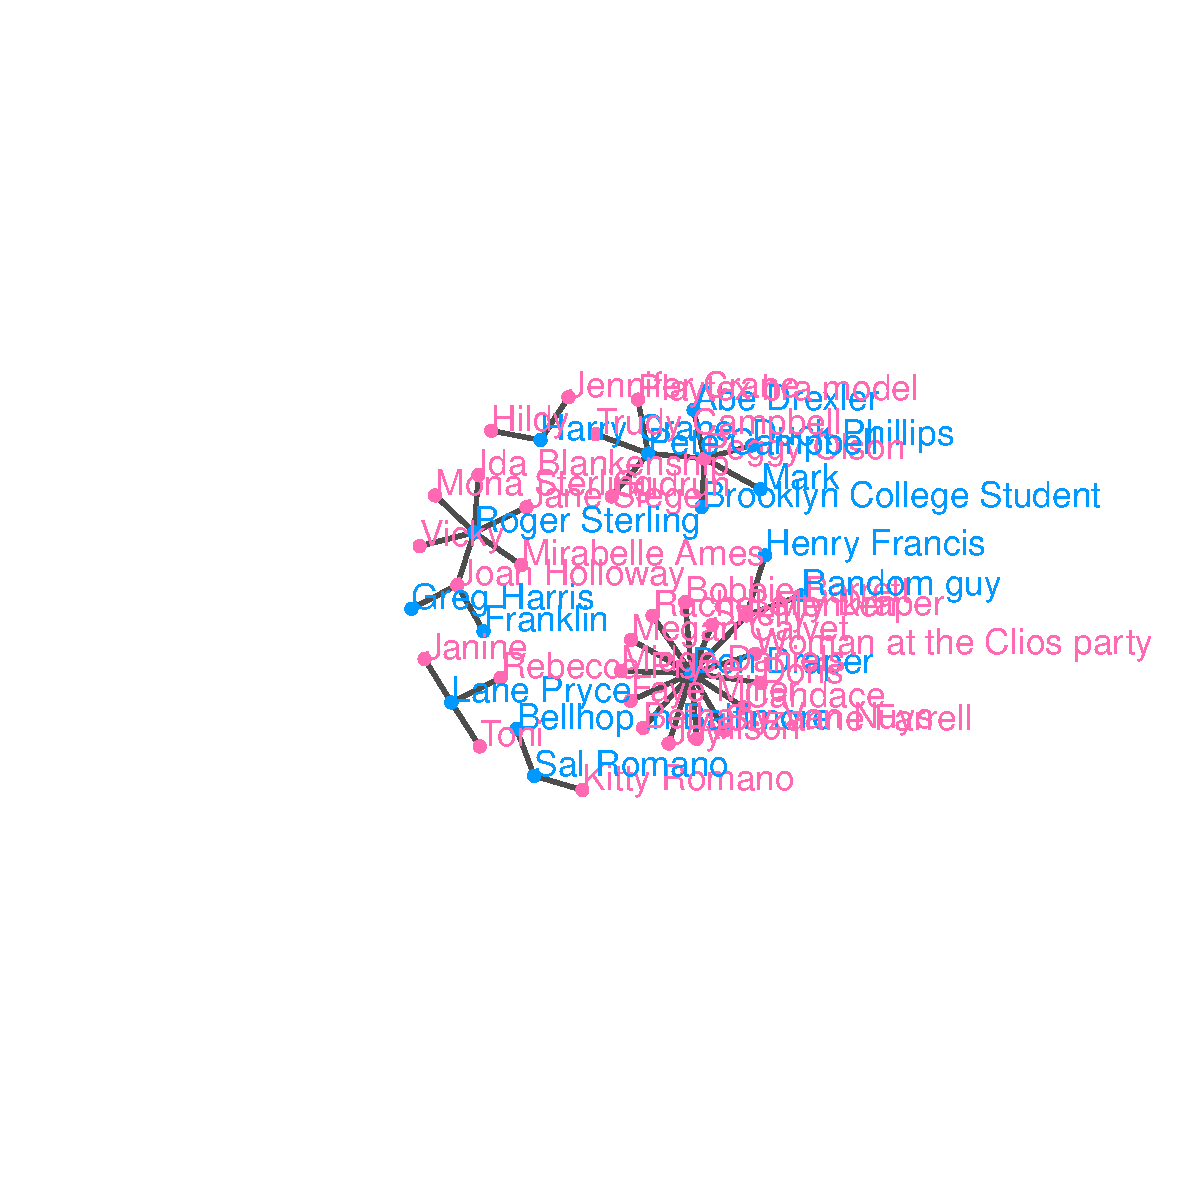
\includegraphics[width=\textwidth]{figure/madmen_ex-1.pdf}
\caption{\label{fig.cap:madmen_ex} Graph of the characters in the show Mad Men who are linked by a romantic relationship.}
\end{figure}
\afterpage{\clearpage}

 In the plot, we can see one central character who has many more relationships than any other character. This vertex represents the main character of the show, Don Draper, who is quite the ``ladies' man."  This fun example shows just how ubiquitous networks are.
\par There are many kinds of networks, and networks are extensively studied across many disciplines.  Many sociologists study social networks, and many biologists study protein networks. As different as these and the many other disciplines that study networks are, they all need the ability to quickly and effectively visualize networks.  We found the current tools to be lacking in this ability, so we chose to fill this gap by adding network plotting capabilities to the popular and widely used \texttt{R} package \texttt{ggplot2}. Just to give an idea of the popularity and the wide-spread use of \texttt{ggplot2}, from January 1, 2015 to March 21, 2015, \texttt{ggplot2} was downloaded over 270,000 times, or approximately 3,454 downloads per day. It has also been downloaded in 189 countries at least once, and in 31 of those countries, including China, Israel, and Colombia, it has been downloaded over 1,000 times\footnote{\texttt{ggplot2} usage statistics taken from \url{http://cran-logs.rstudio.com/}.}. This is the user base we are aiming at by making network visualizations a part of \texttt{ggplot2}.

\par The three necessary elements of any network visualization are the vertices, the edges, and the layout.  But once those three items are visualized, we usually find our visualization to be lacking.  We may want to color the vertices (or edges) by some sort of grouping variable, or we may want to make vertices of degree ten twice the size of vertices of degree five.  Many \texttt{R} packages already exist for network analysis and visualization such as \texttt{igraph} by \citet{igraph}, \texttt{sna} by \citet{sna}, and \texttt{network} by \citet{network.jss, network} but we have found these packages to have unintuitive or burdensome methods for customizing the colors, sizes, etc of the vertices and edges of the network. For instance, the \texttt{igraph} package allows for coloring vertices by groups but the user must assign the colors to each vertex individually as opposed to assigning color by a grouping factor variable. \\


\par The \texttt{GGally} package by \citet{ggally} contains a very useful function written by Fran\c{c}ois Briatte and Moritz Marbach called \texttt{ggnet} that does allow for fairly straightforward customization of these three necessary graph attributes.
Coloring the vertices or edges in a graph is a quick and easy way to visualize grouping and can help with pattern or cluster detection. The vertices in a network and the edges between them compose the structure of a network, and being able to discover patterns among them visually is a key part of network analysis. Viewing multiple layouts of the same network can also help reveal patterns or clusters that would not be discovered when only viewing one layout or analyzing only an adjacency matrix. The \texttt{ggnet} function, however, requires the graph input to be a \texttt{network} object according to the \texttt{network} package.  Our work builds off of the \texttt{ggnet} function and presents an intuitive \texttt{geom} for network visualization within the \texttt{ggplot2} framework, without the need for objects other than simple data frames.

  \subsection{Data Structure}
In order for this geometry to work using data frames, there need to be two separate data frames given to the \texttt{geom\_net} function: one for the edge information and one for the vertex information. The vertex data frame should contain all the relevant vertex information. The only necessary variable is one called \texttt{label} which contains the vertex labels as they are encoded in the edges data set. This will be a formal requirement in the final version of the \texttt{geom\_net} function.  Each row represents one vertex.  Other values of interest, such as grouping variables or degree of each vertex should be stored as columns in this dataframe, with an observation for each vertex.
  \par The edge data frame should contain all the relevant edge information. The only necessary variables are the ``from vertex" and ``to vertex" for each edge in the network. The From and To vertices should match the names of the vertices in the vertex information data frame. The formal names for these columns are \texttt{from\_id} and \texttt{to\_id}, respectively.  Other variables may also be included for each edge, such as the edge weight or grouping variable.  As before, the variables of interest are columns in the data frame and the rows are each edge in the network.

  \subsection{Vertex Aesthetics}

  In our geometry, we want to create all possible vertex aesthetic to mimic the usual aesthetics in \texttt{ggplot2} for points. The \texttt{vcolor} aesthetic can be an identity color (e.g. \texttt{color = "red"}) to change the color of all vertices, or, in the final version, it will take a factor variable which identifies each vertex as belonging to one of several groups, and it colors the vertices of the graph according to this grouping. In the current version, the \texttt{vcolor} aesthetic does not work like a typical color aesthetic in \texttt{ggplot2}. It can, however, take HEX color characters and assign them to different levels of a factor variable. We use the \texttt{RColorBrewer} package to choose the colors for us in this paper \citep{RColorBrewer}. It will also color the vertices along a color gradient according to the different values of some numeric variable such as degree.  The vertex color defaults to black. % are set to the default color palette in \texttt{ggplot2}, and the palette used can be changed in the usual way within the \texttt{ggplot2} framework, by using \texttt{scale\_color\_brewer}.}
  %The \texttt{vcolor} aesthetic operates in the same way as the \texttt{vfill} aesthetic, but it changes the outline color of the vertex instead of the fill color of the vertex, which is in line with the \texttt{ggplot2} use of the \texttt{color} and \texttt{fill} aesthetics.
  The \texttt{vsize} aesthetic can also be set to an identity value to increase or decrease the size of all vertices in the graph, or it can be set to one of any numerical columns in the vertex data frame. Right now, the numerical values are strict point values: if the size of a vertex is two, then it will be two points in diameter. A point is the size of the default fontsize in the \texttt{grid} package. In our final version, the \texttt{vsize} will scale to minimum and maximum values as all other size aesthestics in \texttt{ggplot2} do.  The \texttt{vshape} aesthetic is for changing the shape of the vertices from the default circle to other shapes, like square or triangle.  It also changes the shape of the vertices according to some grouping variable, which is currently required to consist of integer values from 0 to 25.  In the final version, it will be able to change shape based on different levels of a factor variable.  Finally, the \texttt{valpha} aesthetic will change the vertex transparency to a set value, like 1/10 or 0.5.  It operates in exactly the same way as the \texttt{alpha} aesthetic in \texttt{geom\_point}.  This aesthetic is very useful for networks with hundreds or thousands of vertices, which can easily crowd the static visualization. Making the vertices more transparent will better show the underlying structure in the network.

\par Evidently, we created all of these aesthetics to fit in exactly to the \texttt{ggplot2} grammar of graphics. We also created the edge aesthetics in a similar fashion.
  \subsection{Edge Aesthetics}
  Again, our edge aesthetics mimic the familiar \texttt{ggplot2} aesthetics, this time for segments.    The \texttt{ecolor} aesthetic changes the color of all of the edges according to the identity function or can change the color according to HEX colors assigned to levels of a grouping variable.  In the final version, the \texttt{ecolor} aesthetic will automatically color according to levels of a grouping variable or according to a gradient scale associated with a numeric variable.
  The \texttt{elinetype} aesthetic can also be used with a grouping variable to change the line type of each edge in the graph from solid to one of the different types of lines in \texttt{ggplot2}. Currently, the column associated with this aesthetic must be integer valued and take on values from zero to six. In the final version, it will change the edge linetypes according to levels of a grouping variable.  The \texttt{esize} aesthetic can also be set to the weight or probability of each edge, or it can be changed for all edges with the identity function. The associated column can take on any numerical values, and currently maps the values directly to points, just like the \texttt{vsize} aesthetic. In the final version, this aesthetic will work exactly like the sizing in \texttt{ggplot2}, by scaling sizes to the minimum and maximum values. This is one of two ways to visualize the number of edges between two vertices.  The other way is through the \texttt{ealpha} aesthetic. The \texttt{ealpha} aesthetic can change the edge transparency to a set value on the interval $[0,1]$.  If there are multiple edge connections given between two vertices in the edge data frame, the \texttt{ealpha} aesthetic can be changed to plot opaque lines between vertices with many mutual connections and varying degrees of transparent lines between vertices with only a few or a single connection. This property is also especially useful for large networks with a lot of connections or with vertices of relatively high degree. Finally, we will add an \texttt{elabel} aesthetic to print the name or number assigned to each edge on or next to it.  This aesthetic will be very useful for visualizing random graphs or Markov processes where each edge probability is of interest.

  \subsection{Other Arguments}
  Similar to the other geometries and functions in \texttt{ggplot2}, our geometry takes several arguments outside of the aesthetic mapping parameters.  One such argument is the \texttt{vlabel} argument. The \texttt{vlabel} aesthetic is a logical value that, if set to \texttt{TRUE} prints the name or number associated with each vertex in the \texttt{label} column in order to identify it on the plot.  In the final version of this geometry, we will add capabilities to adjust the size and positioning of the labels. For the moment, the color is set to the vertex color, the size is set to twice the vertex size, and all other possible parameters are set to their defaults in \texttt{geom\_text()}. The \texttt{vlabel} argument is most useful for smaller network objects where all vertex names can be printed on their corresponding vertices and still be read clearly.  Next, the \texttt{directed} argument is a logical value that identifies whether or not the network is directed.  When this value is true, arrows are created on the end of the line segment that corresponds to the \texttt{to\_id} value for each edge.  The arrows match the edges in coloring, linetype, and size, and the default length of the arrow is set using the \texttt{unit} function in the \texttt{grid} package to 0.015 of the normalised parent coordinates of the plot.
  Finally, the \texttt{layout} argument takes a character value corresponding to the possible layouts in the \texttt{sna} package that are created by the \texttt{gplot.layout.*()} family of functions.  The default layout is the Kamada-Kawai layout.  This is a force-directed layout for undirected networks \citep{kamadakawai}. There are, however, many other layouts possible.
\begin{table}
\centering
\begin{tabular}{l|p{10cm}}
Layout Name & Description \\
\hline \hline
\texttt{"adj"} & a version of \texttt{"mds"} which scales the raw adjacency matrix \\
\texttt{"circle"}* & places vertices uniformly in a circle \\
\texttt{"circrand"} & places vertices randomly in a circle \\
\texttt{"eigen"} & places vertices based on the eigenstructure of the adjacency matrix \\
\texttt{"fruchtermanreingold"} & uses a variant of Fruchterman and Reingold's force-directed placement algorithm \\
\texttt{"geodist"} & a version of \texttt{"mds"} which scales the matrix of geodesic distances \\
\texttt{"hall"}* &  places vertices based on the last two eigenvectors of the Laplacian of the input matrix \\
\texttt{"kamadakawai"} & generates a vertex layout using a version of the Kamada-Kawai force-directed placement algorithm \\
\texttt{"mds"}  & places vertices based on a metric multidimensional scaling of a specified distance matrix \\
\texttt{"random"} & places vertices randomly \\
\texttt{"segeo"} & a version of \texttt{"mds"} which scales the squared euclidean distances between row-wise geodesic distances \\
\texttt{"seham"} & a version of \texttt{"mds"} which scales the Hamming distance between rows/columns of the adjacency matrix \\
\texttt{"target"} & produces a ``target diagram" or ``bullseye" layout using a force-directed placement algorithm.
\end{tabular}
\caption{All possible layouts to pass to \texttt{geom\_net}.  All descriptions are from \citet{sna}.  Note that the layouts marked with an asterisk (*) are the only layouts that do not take layout parameters.}
\label{table:layouts}
\end{table}

All layouts that \texttt{geom\_net} is currently capable of graphing are listed in table \ref{table:layouts}. The layouts not marked with an asterisk can also take their associated layout parameters.  The \texttt{layout.par} argument takes a list of named parameters.  For instance, if \texttt{layout = "random"}, we can also set \texttt{layout.par = list(dist = "normal")} to change the distribution of vertex placement from the default uniform to Gaussian.

\section{Usage Examples}
In this section, we demonstrate the current capabilities of \texttt{geom\_net} in a series of diverse examples.
  \subsection{Blood Donation}
  In this directed network, there are eight vertices and 27 edges.  The vertices represent the eight different blood types in humans that are most important for donation: the ABO blood types A, B, AB, and O, combined with the RhD positive (+) and negative (-) types. The edges are directed: a person whose blood type is that of a \emph{from} vertex can to donate blood to a person whose blood type is that of a corresponding \emph{to} vertex. In the example below, loops are removed because loops exist on every vertex in this example, as blood between two people of matching ABO and RhD type can always be exchanged.
\begin{knitrout}
\definecolor{shadecolor}{rgb}{0.969, 0.969, 0.969}\color{fgcolor}\begin{kframe}
\begin{alltt}
\hlkwd{ggplot}\hlstd{(}\hlkwc{data} \hlstd{= blood}\hlopt{$}\hlstd{edges,} \hlkwd{aes}\hlstd{(}\hlkwc{from_id} \hlstd{= from,} \hlkwc{to_id} \hlstd{= to))} \hlopt{+}
  \hlkwd{geom_net}\hlstd{(}\hlkwc{vertices} \hlstd{= blood}\hlopt{$}\hlstd{vertices,} \hlkwc{vcolour} \hlstd{=} \hlkwd{I}\hlstd{(}\hlstr{'red'}\hlstd{),} \hlkwc{layout} \hlstd{=} \hlstr{'circle'}\hlstd{,}
           \hlkwc{vlabel} \hlstd{=} \hlnum{TRUE}\hlstd{,} \hlkwc{vsize} \hlstd{=} \hlkwd{I}\hlstd{(}\hlnum{3}\hlstd{),} \hlkwc{directed} \hlstd{=} \hlnum{TRUE}\hlstd{)} \hlopt{+}
  \hlkwd{expand_limits}\hlstd{(}\hlkwc{x} \hlstd{=} \hlkwd{c}\hlstd{(}\hlnum{0}\hlstd{,}\hlnum{1}\hlstd{),} \hlkwc{y} \hlstd{=} \hlkwd{c}\hlstd{(}\hlnum{0}\hlstd{,}\hlnum{1}\hlstd{))} \hlopt{+} \hlstd{theme_net}
\end{alltt}


{\ttfamily\noindent\bfseries\color{errorcolor}{\#\# Error in eval(expr, envir, enclos): could not find function "{}geom\_net"{}}}\end{kframe}
\end{knitrout}
This network is shown in figure \ref{fig.cap:blood_ex}.  Here, we have used the aesthetics \texttt{vcolour} and \texttt{vsize} set to identity values to change the size and color of all vertices. We have also used the \texttt{layout} and \texttt{vlabel} arguments to change the default layout to a circle layout and to print the blood types, respectively. The circle layout places blood types of the same ABO type next to each other and spreads the vertices out far enough to distinguish between the various ``in" and ``out" types.  You can tell clearly from this plot that the O- type is the universal donor: it has out degree of seven and in degree of zero. Additionally, you can see that the AB+ type is the universal recepient, with in degree of seven and out degree of zero. Anyone looking at this plot can quickly determine which type(s) of blood they can receive and which type(s) can receive their blood.
\begin{figure}
\centering
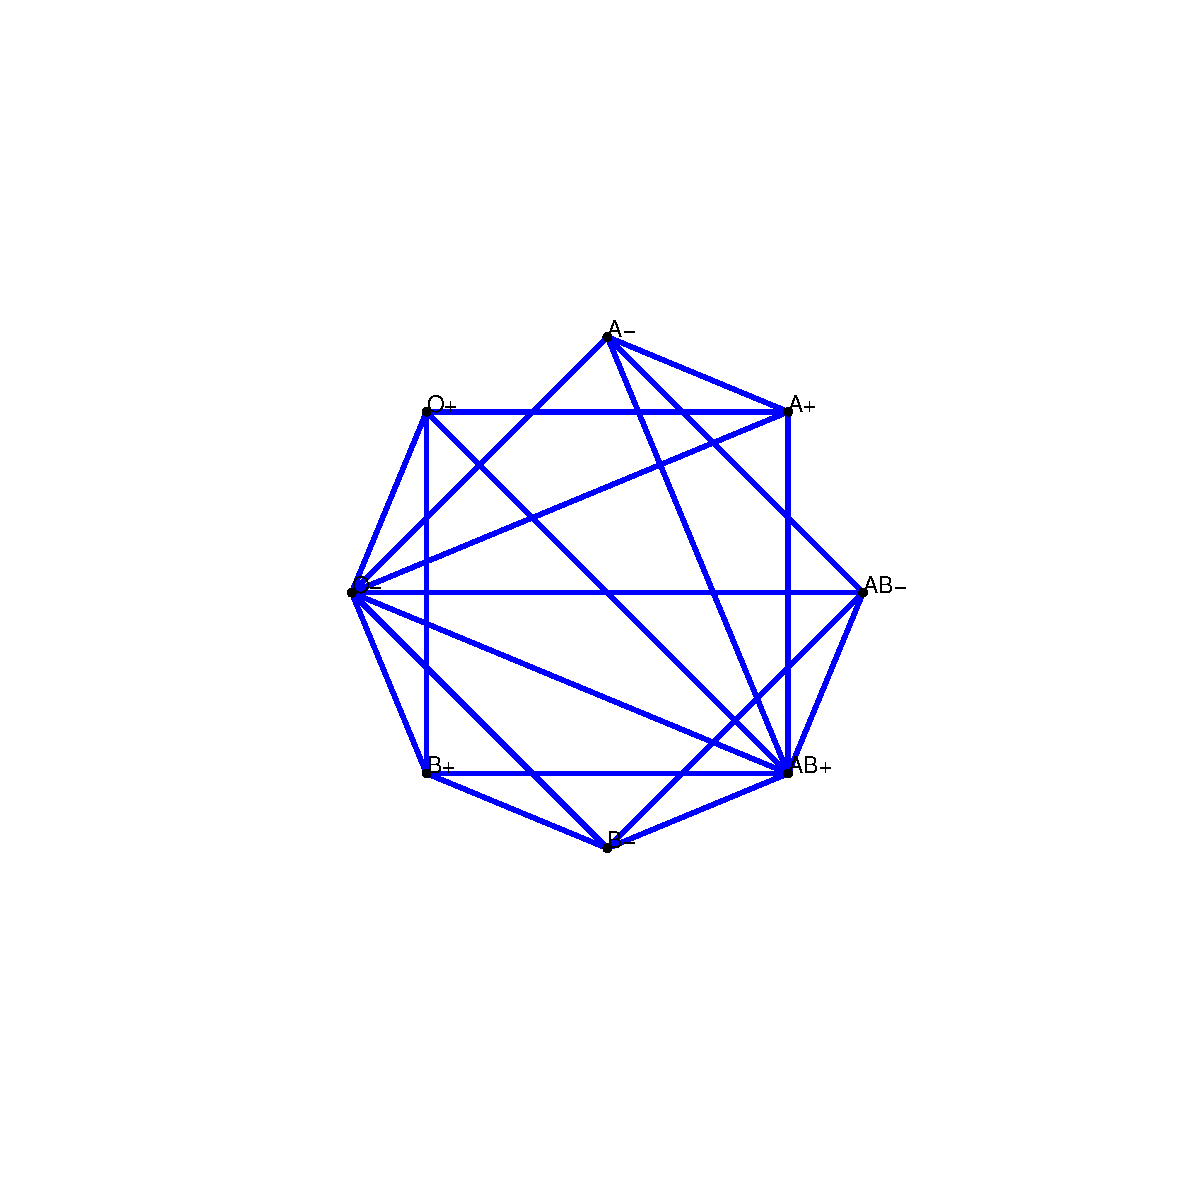
\includegraphics[width=\textwidth]{figure/blood_ex-1.pdf}
\caption{\label{fig.cap:blood_ex} Network of blood donation possibilities in humans by ABO and RhD blood types.}
\end{figure}
\afterpage{\clearpage}

\subsection{Email Network}
  This email network comes from the 2014 VAST Challenge \citep{emailnet}. It is a directed network of emails between company employees with 55 vertices and 9,063 edges. Each vertex is an employee of the company, and each edge is an email sent from one employee to one or more other employees. The arrow of the directed edge points to the recipient(s) of the email. The network contains two business weeks of emails across the entire company. In order to better visualize the structure of the communication network between employees, all emails that were sent out to all employees are removed in the subsequent examples.
\begin{knitrout}
\definecolor{shadecolor}{rgb}{0.969, 0.969, 0.969}\color{fgcolor}\begin{kframe}
\begin{alltt}
\hlkwd{ggplot}\hlstd{(}\hlkwc{data} \hlstd{=} \hlkwd{subset}\hlstd{(email.net, nrecipients} \hlopt{<} \hlnum{54}\hlstd{),} \hlkwd{aes}\hlstd{(}\hlkwc{from_id} \hlstd{= From,} \hlkwc{to_id} \hlstd{= to))} \hlopt{+}
  \hlkwd{geom_net}\hlstd{(}\hlkwc{vertices} \hlstd{= employee,}\hlkwc{ealpha} \hlstd{=} \hlnum{0.1}\hlstd{,} \hlkwc{vsize} \hlstd{=} \hlkwd{I}\hlstd{(}\hlnum{4}\hlstd{),} \hlkwc{directed} \hlstd{=} \hlnum{TRUE}\hlstd{,}
           \hlkwd{aes}\hlstd{(}\hlkwc{vcolour}\hlstd{=cols[}\hlkwd{as.numeric}\hlstd{(CurrentEmploymentType)]))} \hlopt{+}
  \hlkwd{expand_limits}\hlstd{(}\hlkwc{x}\hlstd{=}\hlkwd{c}\hlstd{(}\hlnum{0}\hlstd{,}\hlnum{1}\hlstd{),} \hlkwc{y} \hlstd{=} \hlkwd{c}\hlstd{(}\hlnum{0}\hlstd{,}\hlnum{1}\hlstd{))} \hlopt{+} \hlstd{theme_net}
\end{alltt}


{\ttfamily\noindent\bfseries\color{errorcolor}{\#\# Error in subset(email.net, nrecipients < 54): object 'email.net' not found}}\end{kframe}
\end{knitrout}
\begin{figure}
\centering
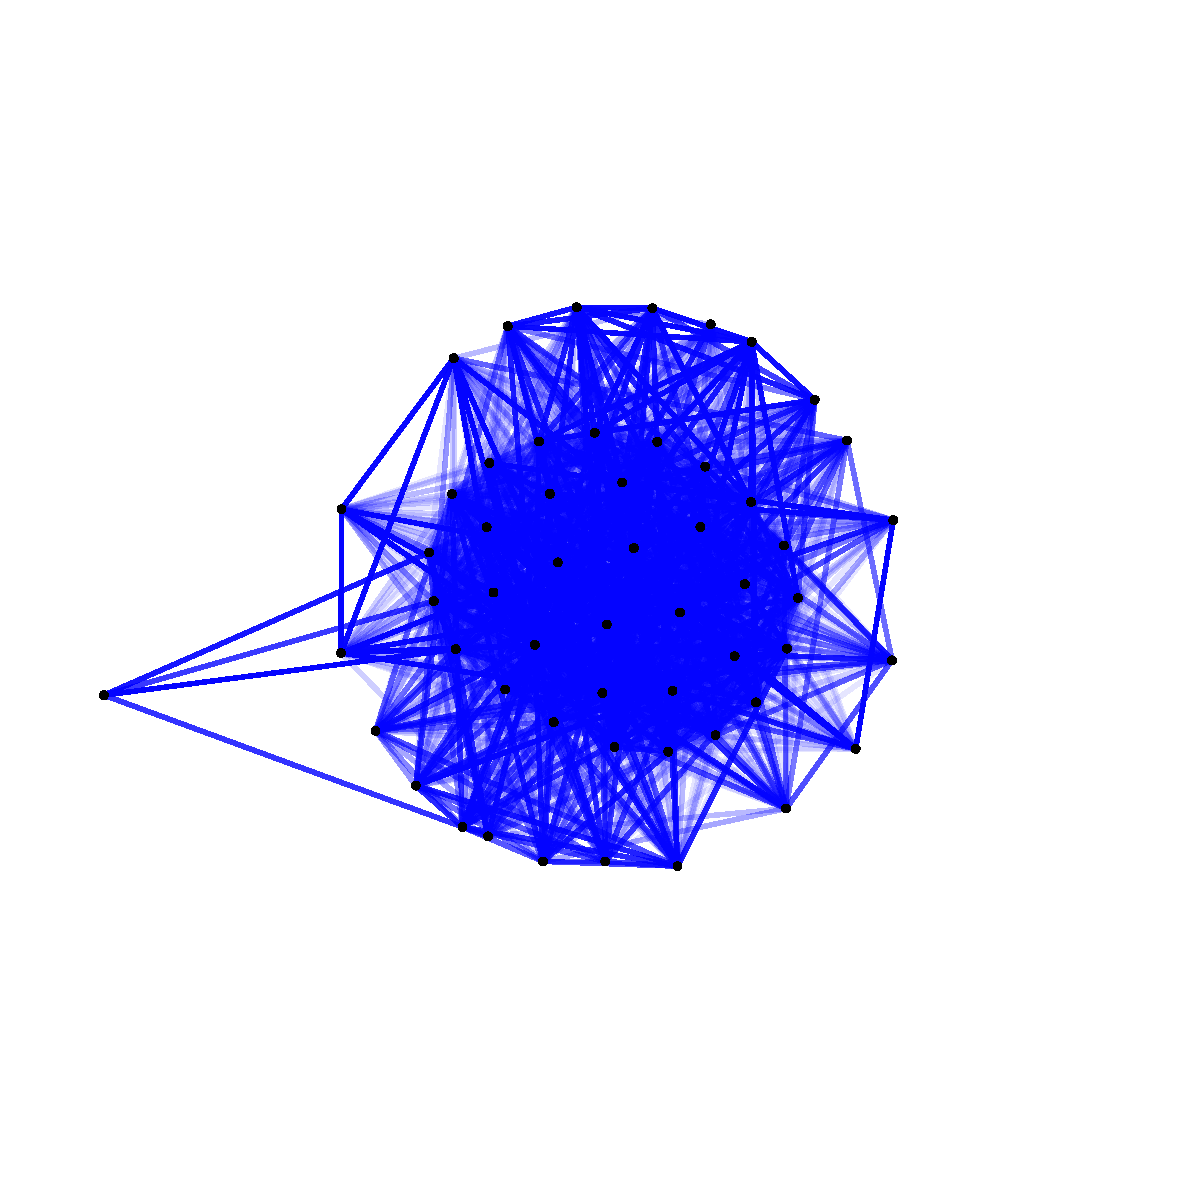
\includegraphics[width=\textwidth]{figure/email_ex-1.pdf}
\caption{\label{fig.cap:email_ex} Email network within a company over a two week period.}
\end{figure}
\afterpage{\clearpage}

This network is plotted in figure \ref{fig.cap:email_ex}.  There are six distinct clusters in this network which almost perfectly correspond to the six different types of employee in this company: administration, engineering, executive, facilities, information technology, and security. Unfortunately, there is currently no legend to associate color with employment type. This will be remedied in the final version of our geometry. Additionally, the edges between employees in the same cluster are much darker than edges between employees in different clusters. This is due to the value of the \texttt{ealpha} aesthetic: more emails between two employees lead to darker edges.  The value is set to 0.1 in this example, so that 10 or more emails between 2 employees results in a completely opaque edge. This pattern of heavy communication between employees of the same type is fairly unsurprising. To make this visualization more interesting and informative, we facet the network by day: each panel in \ref{fig.cap:email_ex_facet} shows the different email networks associated with each day of the week.
\begin{knitrout}
\definecolor{shadecolor}{rgb}{0.969, 0.969, 0.969}\color{fgcolor}\begin{kframe}
\begin{alltt}
\hlkwd{ggplot}\hlstd{(}\hlkwc{data} \hlstd{=} \hlkwd{subset}\hlstd{(email.net, nrecipients} \hlopt{<} \hlnum{54}\hlstd{),} \hlkwd{aes}\hlstd{(}\hlkwc{from_id} \hlstd{= From,} \hlkwc{to_id} \hlstd{= to))} \hlopt{+}
  \hlkwd{geom_net}\hlstd{(}\hlkwc{vertices} \hlstd{= employee,} \hlkwc{ealpha} \hlstd{=} \hlnum{0.2}\hlstd{,} \hlkwc{vsize} \hlstd{=} \hlkwd{I}\hlstd{(}\hlnum{2}\hlstd{),} \hlkwc{directed} \hlstd{=} \hlnum{TRUE}\hlstd{,}
           \hlkwd{aes}\hlstd{(}\hlkwc{vcolour}\hlstd{=cols[}\hlkwd{as.numeric}\hlstd{(CurrentEmploymentType)]))} \hlopt{+}
  \hlkwd{expand_limits}\hlstd{(}\hlkwc{x}\hlstd{=}\hlkwd{c}\hlstd{(}\hlnum{0}\hlstd{,}\hlnum{1}\hlstd{),} \hlkwc{y} \hlstd{=} \hlkwd{c}\hlstd{(}\hlnum{0}\hlstd{,}\hlnum{1}\hlstd{))} \hlopt{+} \hlkwd{facet_wrap}\hlstd{(}\hlopt{~}\hlstd{day,} \hlkwc{nrow} \hlstd{=} \hlnum{2}\hlstd{)} \hlopt{+} \hlstd{theme_net}
\end{alltt}
\end{kframe}
\end{knitrout}
\begin{landscape}
\begin{figure}
\centering
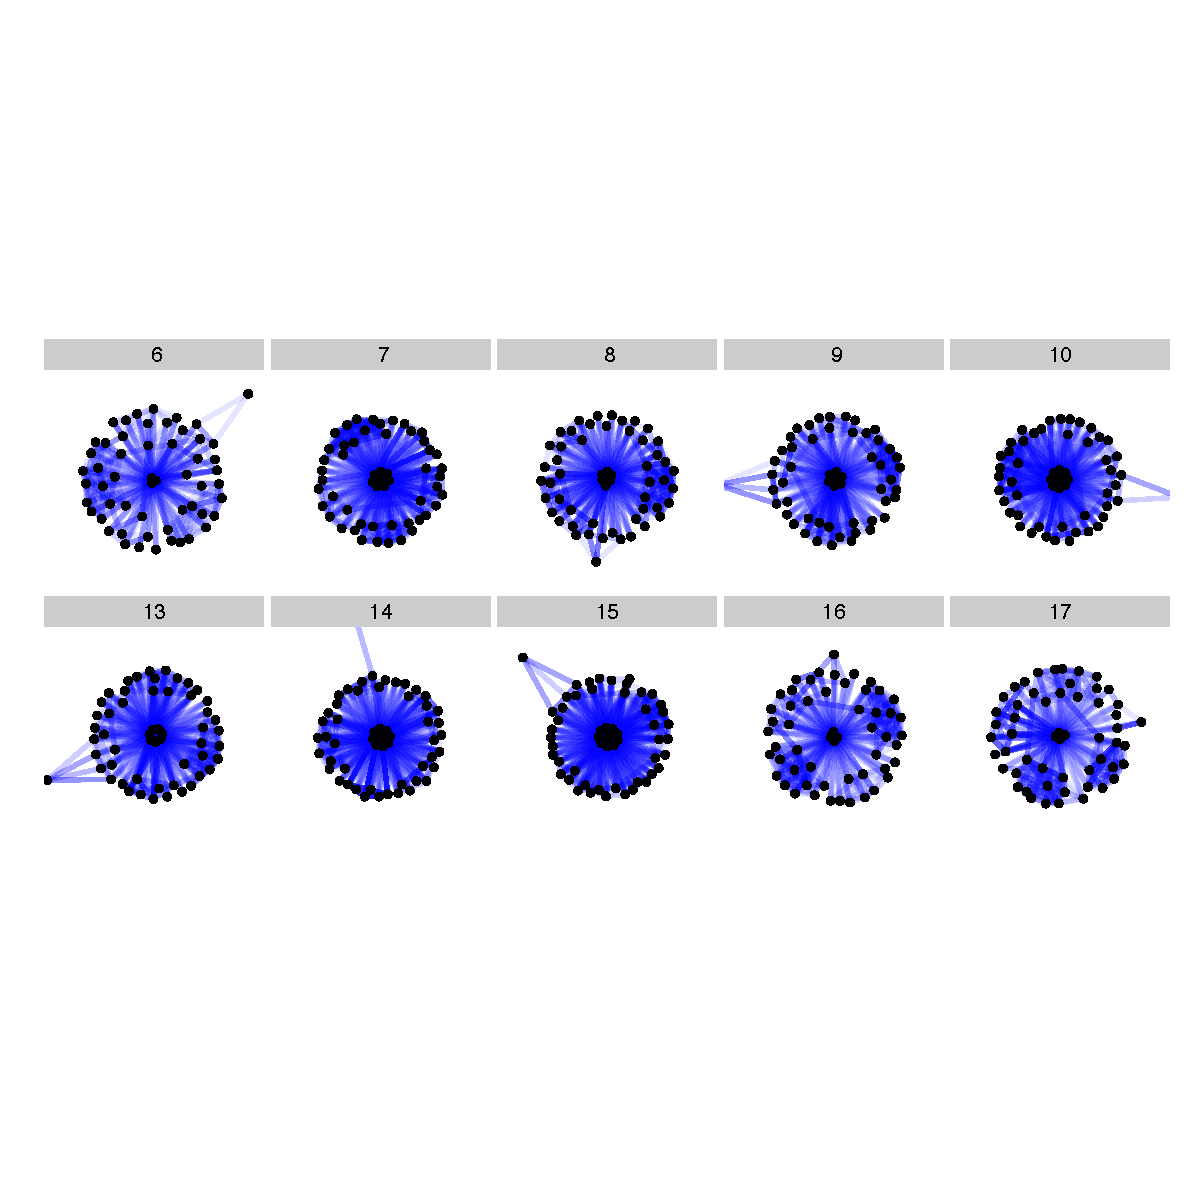
\includegraphics[width=8in]{figure/email_ex_facet-1.pdf}
\caption{\label{fig.cap:email_ex_facet} The same email network as in figure \ref{fig.cap:email_ex} facetted by day of the week.}
\end{figure}
\end{landscape}
This plot is shown in figure \ref{fig.cap: email_ex_facet}. With the facetting, we can see that there are several days where one or more departments do not communicate with any of the other departments. There are only two days, 13 and 15, without any isolated department communications. Facetting is one of the major benefits of creating a geometry for networks in \texttt{ggplot2}.  Facetting quickly separates dense networks into separate subnetworks for easy visual comparison and  analyses.
  \subsection{\texttt{ggplot2} Theme Elements}
This example comes from the \texttt{theme()} help page in the \texttt{ggplot2} documentation \citep{ggplot}.  It is a directed network which shows the structure of the inheritance of theme options in the construction of a \texttt{ggplot2} plot.  There are 53 vertices and 36 edges in this network. Each vertex represents one possible theme option. There is an arrow from one theme option to another if the element represented by the \emph{to} vertex inherits its values from the \emph{from} vertex.  For example, the \texttt{axis.ticks.x} option inherits its value from the \texttt{axis.ticks} value, which inherits its value from the \texttt{line} option.  Thus, setting the \texttt{line} option to a value such as \texttt{element\_blank()} sets the entire inheritance tree to \texttt{element\_blank()}, and no lines appear anywhere on the plot background. Finally, we note that the vertices with no edges were incorporated into the plot by adding their labels to the edges data frame in both the  `from\_id' and `to\_id' columns before passing the edges data frame to \texttt{ggplot}.
\begin{knitrout}
\definecolor{shadecolor}{rgb}{0.969, 0.969, 0.969}\color{fgcolor}\begin{kframe}
\begin{alltt}
\hlkwd{ggplot}\hlstd{(}\hlkwc{data} \hlstd{= theme_elements}\hlopt{$}\hlstd{edges,} \hlkwd{aes}\hlstd{(}\hlkwc{from_id} \hlstd{= parent,} \hlkwc{to_id} \hlstd{= child))} \hlopt{+}
  \hlkwd{geom_net}\hlstd{(}\hlkwc{vertices} \hlstd{= theme_elements}\hlopt{$}\hlstd{vertices,} \hlkwc{directed} \hlstd{=} \hlnum{TRUE}\hlstd{,} \hlkwc{vlabel} \hlstd{=} \hlnum{TRUE}\hlstd{)} \hlopt{+}
  \hlkwd{expand_limits}\hlstd{(}\hlkwc{x} \hlstd{=} \hlkwd{c}\hlstd{(}\hlnum{0}\hlstd{,}\hlnum{1.2}\hlstd{),} \hlkwc{y} \hlstd{=} \hlkwd{c}\hlstd{(}\hlnum{0}\hlstd{,}\hlnum{1}\hlstd{))} \hlopt{+}
  \hlstd{theme_net}
\end{alltt}


{\ttfamily\noindent\bfseries\color{errorcolor}{\#\# Error in eval(expr, envir, enclos): could not find function "{}geom\_net"{}}}\end{kframe}
\end{knitrout}
\begin{figure}
\centering
\includegraphics[width=\textwidth]{figure/theme_ex-1.pdf}
\caption{\label{fig.cap:theme_ex} Inheritance structure of \texttt{ggplot2} theme elements. This is a recreation of the graph found at \protect\url{http://docs.ggplot2.org/current/theme.html}.}
\end{figure}
\afterpage{\clearpage}

The inheritance structure is plotted in figure \ref{fig.cap:theme_ex}.  In this plot, it is easy to quickly determine the parent and child vertices. Using this plot made creation of the \texttt{theme\_net} object used throughout these examples very simple. We just made set each of the major parent elements, \texttt{text}, \texttt{rect}, and \texttt{line} to \texttt{element\_blank()} and then set the aspect ratio equal to one.
  \subsection{Mad Men Networks}
  The following code creates the network example given in the introduction. We changed the vertex size and edge color for all vertices and edges, included vertex labels, and colored the vertices according to the character's gender.
\begin{knitrout}
\definecolor{shadecolor}{rgb}{0.969, 0.969, 0.969}\color{fgcolor}\begin{kframe}
\begin{alltt}
\hlkwd{ggplot}\hlstd{(}\hlkwc{data} \hlstd{= madmen}\hlopt{$}\hlstd{edges,} \hlkwd{aes}\hlstd{(}\hlkwc{from_id} \hlstd{= Name1,} \hlkwc{to_id} \hlstd{= Name2))} \hlopt{+}
  \hlkwd{geom_net}\hlstd{(}\hlkwc{vertices} \hlstd{= madmen}\hlopt{$}\hlstd{vertices,} \hlkwc{vsize}\hlstd{=}\hlnum{3}\hlstd{,} \hlkwc{vlabel}\hlstd{=} \hlnum{TRUE}\hlstd{,} \hlkwc{ecolour}\hlstd{=}\hlstr{"grey30"}\hlstd{,}
           \hlkwd{aes}\hlstd{(}\hlkwc{vcolour}\hlstd{=}\hlkwd{c}\hlstd{(} \hlstr{"#FF69B4"}\hlstd{,} \hlstr{"#0099ff"}\hlstd{)[}\hlkwd{as.numeric}\hlstd{(Gender)]))} \hlopt{+}
  \hlkwd{expand_limits}\hlstd{(}\hlkwc{x} \hlstd{=} \hlkwd{c}\hlstd{(}\hlnum{0}\hlstd{,}\hlnum{1.25}\hlstd{),} \hlkwc{y} \hlstd{=} \hlkwd{c}\hlstd{(}\hlnum{0}\hlstd{,}\hlnum{1}\hlstd{))} \hlopt{+} \hlstd{theme_net}
\end{alltt}
\end{kframe}
\end{knitrout}
 There is another Mad Men network included in the \texttt{gcookbook} package \citep{madmen}. It is a directed network, also of romantic relationships between characters, but it also includes advances made by one character that were rejected by the other.  For example, Roger Sterling made advances toward Betty Draper, but Betty refused him, and so there is a directed edge going from Roger to Betty, but not from Betty to Roger.  If the advance is reciprocated, like between Sal Romano and the Bellhop, there are two directed edges between the two vertices.
\begin{knitrout}
\definecolor{shadecolor}{rgb}{0.969, 0.969, 0.969}\color{fgcolor}\begin{kframe}
\begin{alltt}
\hlkwd{ggplot}\hlstd{(}\hlkwc{data} \hlstd{= mm.directed}\hlopt{$}\hlstd{edges,} \hlkwd{aes}\hlstd{(}\hlkwc{from_id} \hlstd{= Name1,} \hlkwc{to_id} \hlstd{= Name2))} \hlopt{+}
  \hlkwd{geom_net}\hlstd{(}\hlkwc{vertices} \hlstd{= mm.directed}\hlopt{$}\hlstd{vertices,} \hlkwc{directed} \hlstd{= T,} \hlkwc{vlabel} \hlstd{= T,}
           \hlkwc{vsize} \hlstd{=} \hlkwd{I}\hlstd{(}\hlnum{2.5}\hlstd{),} \hlkwc{layout} \hlstd{=} \hlstr{'fruchtermanreingold'}\hlstd{,}
           \hlkwd{aes}\hlstd{(}\hlkwc{vcolour}\hlstd{=}\hlkwd{c}\hlstd{(} \hlstr{"#FF69B4"}\hlstd{,} \hlstr{"#0099ff"}\hlstd{)[}\hlkwd{as.numeric}\hlstd{(Gender)]))} \hlopt{+}
  \hlkwd{expand_limits}\hlstd{(}\hlkwc{x} \hlstd{=} \hlkwd{c}\hlstd{(}\hlnum{0}\hlstd{,}\hlnum{1.1}\hlstd{),} \hlkwc{y} \hlstd{=} \hlkwd{c}\hlstd{(}\hlnum{0}\hlstd{,}\hlnum{1}\hlstd{))} \hlopt{+} \hlstd{theme_net}
\end{alltt}


{\ttfamily\noindent\bfseries\color{errorcolor}{\#\# Error in ggplot(data = mm.directed\$edges, aes(from\_id = Name1, to\_id = Name2)): object 'mm.directed' not found}}\end{kframe}
\end{knitrout}
\begin{figure}
\centering
\includegraphics[width=\textwidth]{figure/madmen2_ex-1.pdf}
\caption{\label{fig.cap:madmen2_ex} A directed network of relationships in Mad Men.}
\end{figure}
This network is shown in figure \ref{fig.cap:madmen2_ex}.  This network is much more connected than the previous Mad Men example.  It also allows us to see much more of the drama in the show. For instance, you can see that Roger made advances towards Betty, his business partner's wife, which is much more scandalous than what we can see in the first network.

  \subsection{College Football}
  This next example comes from M.E.J. Newman's network data web page \citep{football}.  It is an undirected network consisting of all regular season college football games played between Division I schools in Fall of 2000.  There are 115 vertices and 613 edges: each vertex represents a school, and an edge represents a game played between two schools. There is an additional variable in the vertex data frame corresponding to the conference each team belongs to, and there is an additional variable in the edge data frame that is equal to one if the game occured between teams in the same conference or zero if the game occured between teams in different conferences.
\begin{knitrout}
\definecolor{shadecolor}{rgb}{0.969, 0.969, 0.969}\color{fgcolor}\begin{kframe}
\begin{alltt}
\hlstd{colors} \hlkwb{<-} \hlkwd{brewer.pal}\hlstd{(}\hlnum{12}\hlstd{,} \hlkwc{name} \hlstd{=} \hlstr{'Paired'}\hlstd{)}
\hlkwd{ggplot}\hlstd{(}\hlkwc{data} \hlstd{= football}\hlopt{$}\hlstd{edges,} \hlkwd{aes}\hlstd{(}\hlkwc{from_id} \hlstd{= from,} \hlkwc{to_id} \hlstd{= to,}
                                  \hlkwc{elinetype} \hlstd{= in.conf} \hlopt{+} \hlnum{1}\hlstd{))} \hlopt{+}
  \hlkwd{geom_net}\hlstd{(}\hlkwc{vertices} \hlstd{= football}\hlopt{$}\hlstd{vertices,} \hlkwc{ealpha} \hlstd{=} \hlnum{0.3}\hlstd{,} \hlkwc{vsize} \hlstd{=} \hlnum{2}\hlstd{,} \hlkwc{vlabel} \hlstd{=} \hlnum{TRUE}\hlstd{,}
           \hlkwd{aes}\hlstd{(}\hlkwc{vcolour}\hlstd{=colors[}\hlkwd{as.numeric}\hlstd{(}\hlkwd{factor}\hlstd{(value))]))} \hlopt{+}
  \hlkwd{expand_limits}\hlstd{(}\hlkwc{x} \hlstd{=} \hlkwd{c}\hlstd{(}\hlnum{0}\hlstd{,}\hlnum{1}\hlstd{),} \hlkwc{y} \hlstd{=} \hlkwd{c}\hlstd{(}\hlnum{0}\hlstd{,}\hlnum{1}\hlstd{))} \hlopt{+} \hlstd{theme_net}
\end{alltt}


{\ttfamily\noindent\bfseries\color{errorcolor}{\#\# Error in eval(expr, envir, enclos): could not find function "{}geom\_net"{}}}\end{kframe}
\end{knitrout}
The network of football games is given in figure \ref{fig.cap:football_ex}. Here, we have changed the \texttt{elinetype} aesthetic to correspond to games that occur between teams in the same conference or different conferences.  These lines are dotted and solid, respectively. We have also assigned a different color to each conference, and the vertices and their labels are colored according to their conference. This coloring and changing of the linetypes make the structure of the game network easier to view.  There is one conference consisting of Navy, Notre Dame, Utah State, Central Florida, and Connecticut, which is spread out all over the network, whereas most other conferences' teams are all very close to each other because they play within conference much more than they play out of conference.  At the time, these five schools were all independents and did not have a home conference.  Without the coloring capability, we would not have been able to pick out that difference as easily.
\begin{figure}
\centering
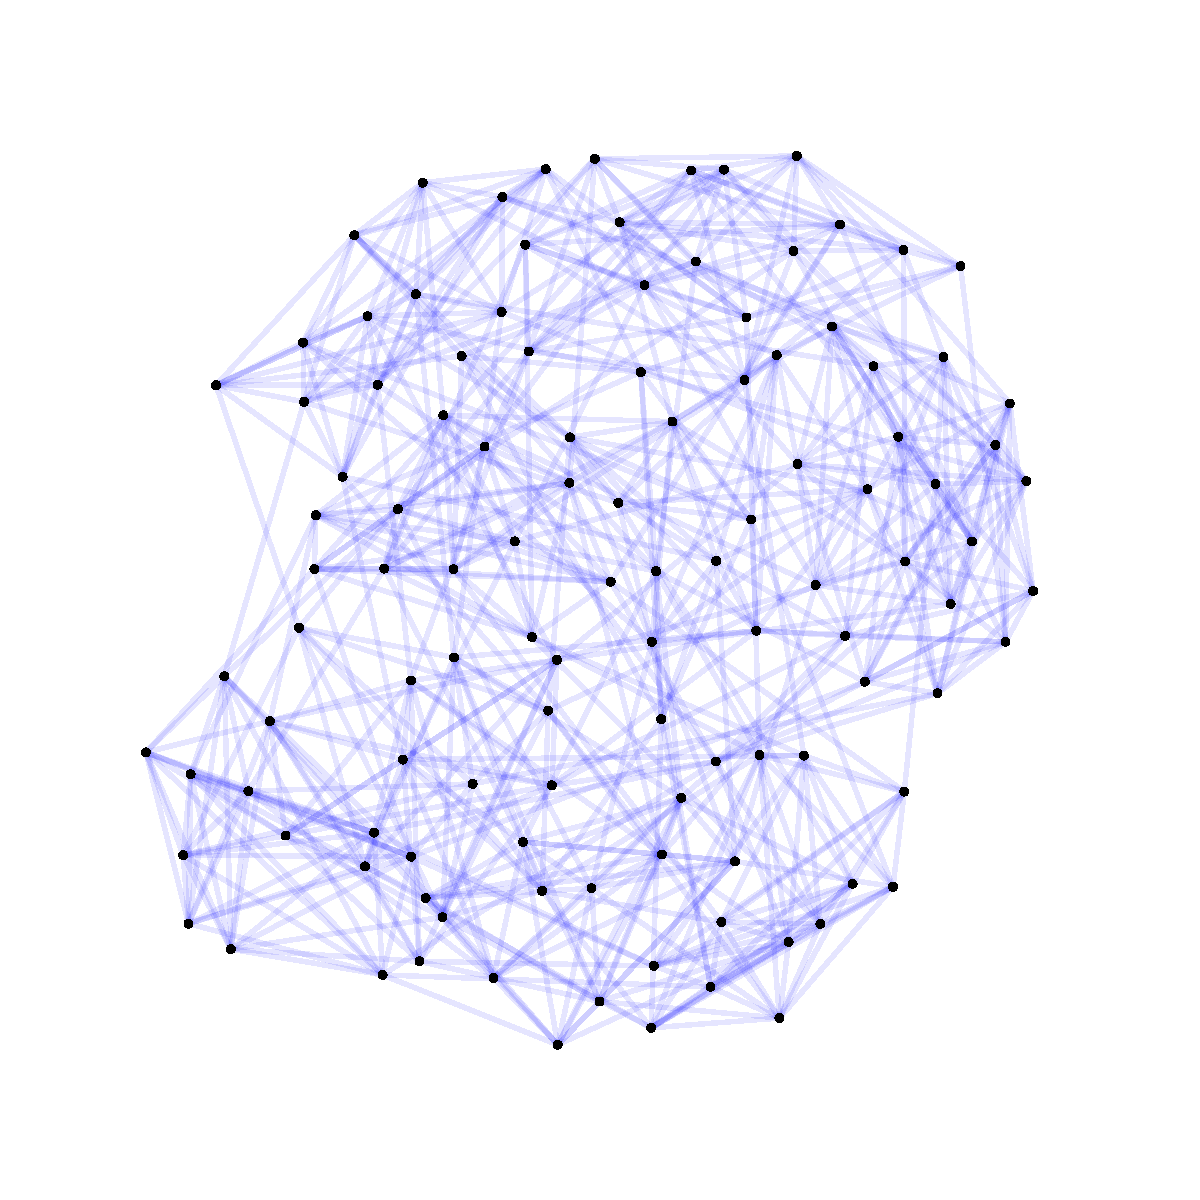
\includegraphics[width=\textwidth]{figure/football_ex-1.pdf}
\caption{\label{fig.cap:football_ex} The network of regular season Division I college football games in the season of fall 2000. The vertices and their labels are colored by conference.}
\end{figure}
\afterpage{\clearpage}

  \subsection{Les Mis\'{e}rables}
  This next network comes from \citet{lesmis}. It is an undirected network of coappearances of characters in Victor Hugo's \emph{Les Mis\'{e}rables}.  There are 77 vertices representing each of the 77 characters in the book, and an edge connects two vertices if those two characters appear in the same chapter of the book.  There are 254 edges in this network. The edges are also weighted by the number of coappearances. The largest weighting is 31, between the characters Jean Valjean and Cosette.  This network is shown in figure \ref{fig.cap:lesmis_ex}. This network reveals many important character groups, as well as the main characters in the story.  The main characters are the ones with high degree, like Valjean, Cosette, and Javert.  There is an extremely wide edge connecting Valjean and Cosette, which implies that they are strongly connected; in fact, Cosette is Valjean's adopted daughter.
\begin{knitrout}
\definecolor{shadecolor}{rgb}{0.969, 0.969, 0.969}\color{fgcolor}\begin{kframe}
\begin{alltt}
\hlkwd{ggplot}\hlstd{(}\hlkwc{data} \hlstd{= lesmis}\hlopt{$}\hlstd{edges,} \hlkwd{aes}\hlstd{(}\hlkwc{from_id} \hlstd{= from,} \hlkwc{to_id} \hlstd{= to,}
                                \hlkwc{esize} \hlstd{= value}\hlopt{/}\hlkwd{mean}\hlstd{(value)))} \hlopt{+}
  \hlkwd{geom_net}\hlstd{(}\hlkwc{vertices} \hlstd{= lesmis}\hlopt{$}\hlstd{vertices,} \hlkwc{ealpha} \hlstd{=} \hlnum{7}\hlopt{/}\hlnum{10}\hlstd{,}
           \hlkwc{vcolour} \hlstd{=} \hlkwd{I}\hlstd{(}\hlstr{"red"}\hlstd{),} \hlkwc{vsize} \hlstd{=} \hlkwd{I}\hlstd{(}\hlnum{2.5}\hlstd{),}
           \hlkwc{layout} \hlstd{=} \hlstr{'fruchtermanreingold'}\hlstd{,} \hlkwc{vlabel}\hlstd{=}\hlnum{TRUE}\hlstd{)} \hlopt{+}
  \hlkwd{expand_limits}\hlstd{(}\hlkwc{x} \hlstd{=} \hlkwd{c}\hlstd{(}\hlnum{0}\hlstd{,}\hlnum{1.1}\hlstd{),} \hlkwc{y} \hlstd{=} \hlkwd{c}\hlstd{(}\hlnum{0}\hlstd{,}\hlnum{1}\hlstd{))} \hlopt{+} \hlstd{theme_net}
\end{alltt}


{\ttfamily\noindent\bfseries\color{errorcolor}{\#\# Error in eval(expr, envir, enclos): could not find function "{}geom\_net"{}}}\end{kframe}
\end{knitrout}
\begin{figure}
\centering
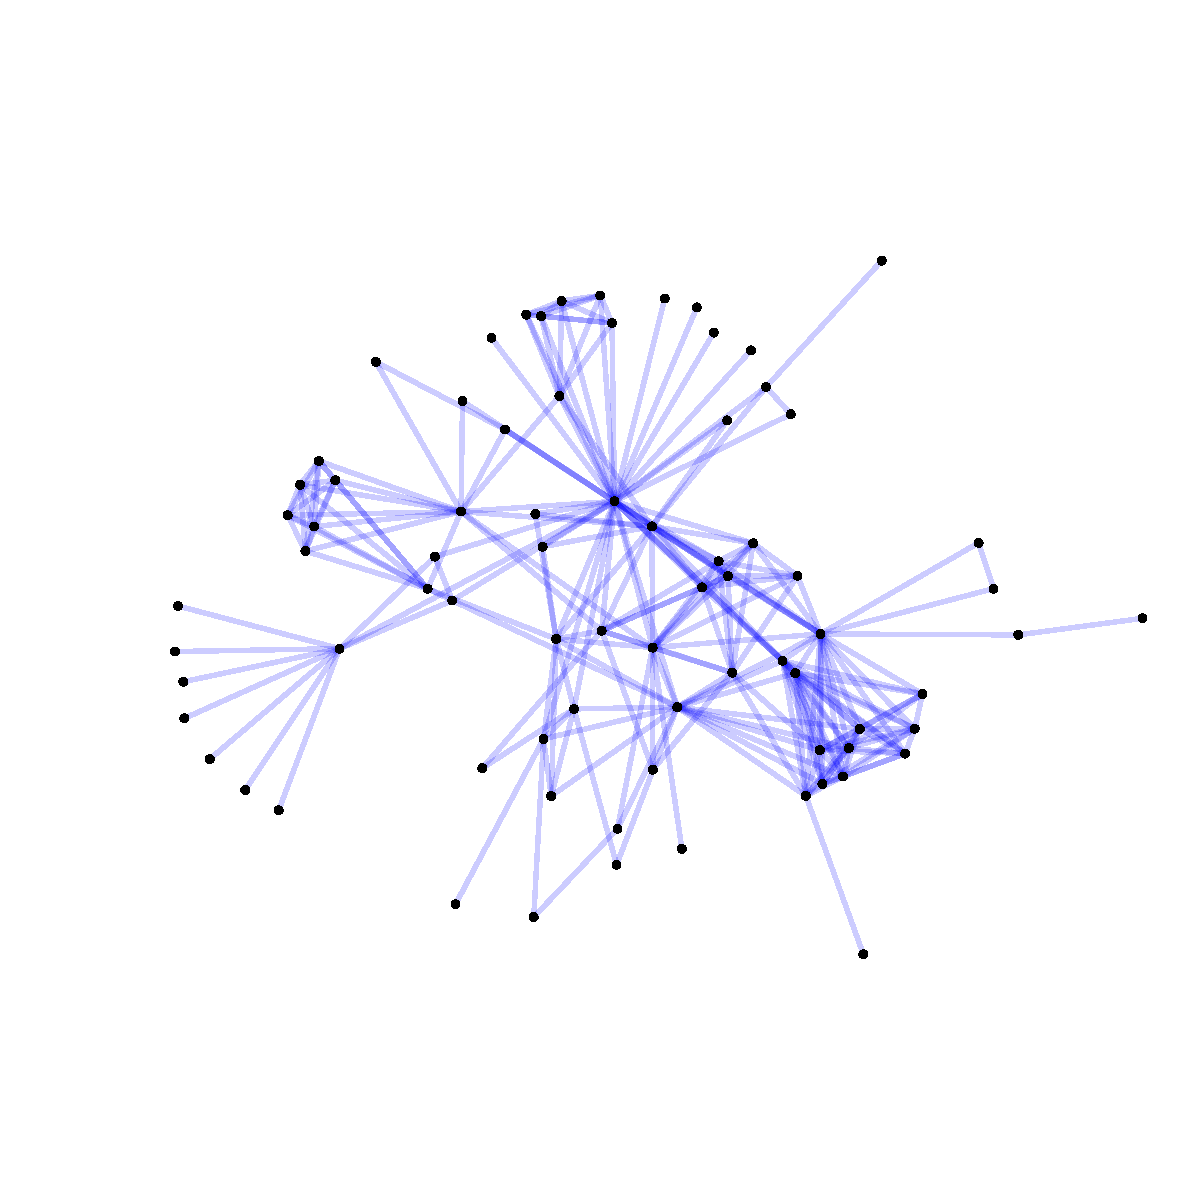
\includegraphics[width=\textwidth]{figure/lesmis_ex-1.pdf}
\caption{\label{fig.cap:lesmis_ex} Co-appearance network of characters in Victor Hugo's \emph{Les Mis\'{e}rables}.}
\end{figure}
\afterpage{\clearpage}

  \subsection{Protein Interaction Network in Yeast}
  This example of a protein interaction network comes from \citet{protein}. It is the complete protein-protein interaction network in the yeast species \emph{S. cerevisiae}. There are 1,870 proteins that make up the vertices of this network, and there are 2,240 edges between them.  These edges represent ``direct physical interactions" between any 2 proteins \citep[][p. 42]{protein}. Because the network is very large, we randomly sampled 500 interactions and their associated proteins to plot it in figure \ref{fig.cap:yeast_ex}.  We also demonstrate the layout capabilities by changing the layout to random and setting the distribution to \texttt{"uniang"}, which is a  ``gaussian donut" layout.  Indeed, we see a nearly round area in the middle of the graph where the layout parameter has forced there to be no vertices.

\begin{knitrout}
\definecolor{shadecolor}{rgb}{0.969, 0.969, 0.969}\color{fgcolor}\begin{kframe}


{\ttfamily\noindent\bfseries\color{errorcolor}{\#\# Error in eval(expr, envir, enclos): object 'yeast' not found}}

{\ttfamily\noindent\bfseries\color{errorcolor}{\#\# Error in eval(expr, envir, enclos): object 'sample.edges' not found}}\end{kframe}
\end{knitrout}
\begin{knitrout}
\definecolor{shadecolor}{rgb}{0.969, 0.969, 0.969}\color{fgcolor}\begin{kframe}
\begin{alltt}
\hlkwd{ggplot}\hlstd{(}\hlkwc{data} \hlstd{= yeast.samp}\hlopt{$}\hlstd{edges,} \hlkwd{aes}\hlstd{(}\hlkwc{from_id} \hlstd{= V1,} \hlkwc{to_id} \hlstd{= V2))} \hlopt{+}
  \hlkwd{geom_net}\hlstd{(}\hlkwc{vertices} \hlstd{= yeast.samp}\hlopt{$}\hlstd{vertices,} \hlkwc{ealpha} \hlstd{=} \hlnum{.25}\hlstd{,} \hlkwc{valpha} \hlstd{=} \hlnum{.5}\hlstd{,}
           \hlkwc{vcolour} \hlstd{=} \hlstr{'magenta'}\hlstd{,} \hlkwc{layout} \hlstd{=} \hlstr{'random'}\hlstd{,}
           \hlkwc{layout.par} \hlstd{=} \hlkwd{list}\hlstd{(}\hlkwc{dist} \hlstd{=} \hlstr{'uniang'}\hlstd{))} \hlopt{+}
  \hlkwd{expand_limits}\hlstd{(}\hlkwc{x} \hlstd{=} \hlkwd{c}\hlstd{(}\hlnum{0}\hlstd{,}\hlnum{1}\hlstd{),} \hlkwc{y} \hlstd{=} \hlkwd{c}\hlstd{(}\hlnum{0}\hlstd{,}\hlnum{1}\hlstd{))} \hlopt{+} \hlstd{theme_net}
\end{alltt}


{\ttfamily\noindent\bfseries\color{errorcolor}{\#\# Error in ggplot(data = yeast.samp\$edges, aes(from\_id = V1, to\_id = V2)): object 'yeast.samp' not found}}\end{kframe}
\end{knitrout}

\begin{figure}
\centering
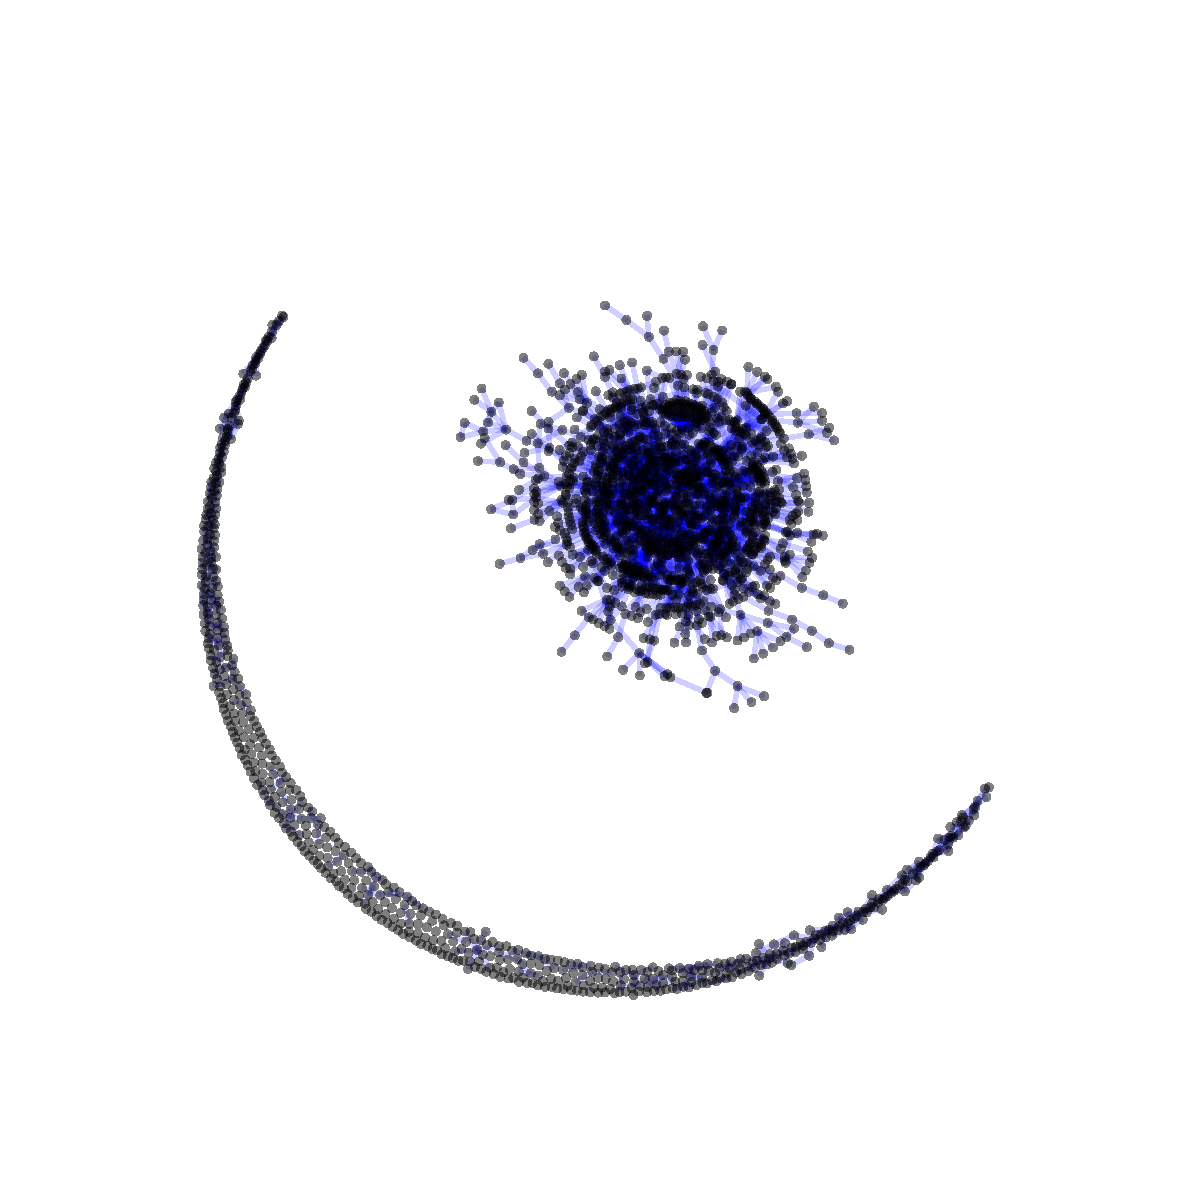
\includegraphics[width=\textwidth]{figure/yeast_ex-1.pdf}
\caption{\label{fig.cap:yeast_ex} A subset of the complete protein-protein interaction network in \emph{S. cerevisiae}. The layout is random.}
\end{figure}
\afterpage{\clearpage}


\section{Technical Details}

In order to construct the \texttt{geom} in \texttt{ggplot2}, we needed two \texttt{R} script files: a `stat' file and a `geom' file. The stat file performs all the necessary calculations on the two input data frames, and the geom file performs the drawing of the network.
  \subsection{Creating \texttt{stat\_net}}
  In order to plot the network with only the edge connections and vertex names, we relied on the \texttt{sna} and \texttt{network} packages \citep{sna, network.jss}. First, we used the edges data frame to construct a network object with the \texttt{as.network()} function, then constructed an adjacency matrix from that network using the \texttt{as.matrix.network.adjacency()} function.  This adjacency matrix is then passed to the chosen \texttt{gplot.layout.*()} function from the \texttt{sna} package.  \emph{When the layout argument is changed in the \texttt{geom\_net()} function, the corresponding \texttt{gplot.layout.*()} function in \texttt{sna} is called with a \texttt{do.call()} statement.} This layout function produces a matrix of coordinates of the vertices, which we then transform into a data frame containing the coordinates of the edges using the \texttt{as.matrix.network.edgelist()} function in \texttt{network}.  We are grateful to Moritz Marbach for his \texttt{gplot()} function which we used when creating this process \citep{marbach}.  At the end of the previous routine, we have a data frame with \texttt{x, y, xend,} and \texttt{yend} columns describing the edges and another data frame with \texttt{x,y} columns describing the vertices.  These two data frames, along with the many \texttt{aes()} and other argument options get passed on to the actual network geometry for drawing.
   \subsection{\texttt{stat\_net} Usage}

  The usage of the \texttt{stat\_net} arguments is as follows:
  \begin{itemize}
  \item The \texttt{mapping} argument is the aesthetic mapping. Currently, there is no reason to ever change it from \texttt{NULL}.
  \item The \texttt{data} argument is the edges data frame.  This is sent to \texttt{stat\_net} through the \texttt{ggplot()} function.
  \item The \texttt{vertices} argument is the vertex data frame. This is sent to \texttt{stat\_net} through the \texttt{geom\_net} function.
  \item The \texttt{geom} argument is the geometric object used to plot the data. It is by default set to \texttt{net}.
  \item The \texttt{position} argument is set to \texttt{identity} because we wish to plot the network as-is, with no adjustments.
  \item na.rm
  \end{itemize}
  \texttt{stat\_net} also accepts the following aesthetic values, none of which are required:
  \begin{itemize}
  \item The \texttt{layout} aesthetic is the layout algorithm to use to place the vertices of the network.  The default is the Kamada-Kawai algorithm, and there are other options listed in \ref{table:layouts}.
  \item The \texttt{layout.par} aesthetic is the layout arguments to pass to the layout function.  It is set to \texttt{NA} by default, in which case the algorithm uses its set defaults in the \texttt{sna} package. This aesthetic takes a list of parameters according to the documentation by \citet{sna}.
  \end{itemize}

  \subsection{Creating \texttt{geom\_net}}
  We constructed \texttt{geom\_net} using the drawing capabilities of the \texttt{geom\_point}, \texttt{geom\_line}, \emph{and \texttt{geom\_text}} functions that were already in \texttt{ggplot2}.  Using these capabilities, we were able to seamlessly incorporate our network geometry into the \texttt{ggplot2} structure. We took our edges data frame and used that as our input to the \texttt{GeomSegment} draw function to add a layer of segments to the plot.  Then, on top of that, we plot the vertices by passing our vertex data frame to the \texttt{GeomPoint} draw function to construct a point layer for the vertices. Finally, we use the \texttt{GeomText} draw function to add the vertex labels when the \texttt{vlabel} argument is TRUE. This adds a layer of text on top of the other two layers. We added an if/else statement in the \texttt{draw} function which created a labeling layer which is \texttt{NULL} if \texttt{vlabel = FALSE}, which is the default. We then created a new data frame for the label layer. This allows the vertex properties to be propogated through to the labels, including size and color. Finally, we added another if/else statement for the \texttt{directed} argument.  This adds arrow arguments to the edges data frame which will put arrows pointing toward the ``to" vertex in a directed network corresponding to the \texttt{to\_id} value in the edges data frame.

   \subsection{\texttt{geom\_net} Usage}

  The usage of the \texttt{geom\_net} arguments is as follows:
  \begin{itemize}
  \item The \texttt{mapping} argument is the aesthetic mapping. It is constructed with \texttt{aes()} according to the aesthetic values that can be passed to \texttt{geom\_net}.
  \item The \texttt{data} argument is the edges data frame.  There is usually no need to use it in \texttt{geom\_net()} because it will have already been provided in the \texttt{ggplot()} function.
  \item The \texttt{vertices} argument is the vertex data frame. The vertex data frame should be provided to this argument in \texttt{geom\_net}. This data frame is required to have a column named \texttt{label} providing the labels of all vertices in the network.
  \item The \texttt{vlabel} argument is a logical value which plots the label layer on top of the edge and vertex layers when it is set to \texttt{TRUE}.
  \item The \texttt{directed} argument is a logical value which adds arrows to the edge layer pointing to the \texttt{to\_id} vertex when it is set to \texttt{TRUE}.
  \item The \texttt{stat} argument is the statistical transformation used on the data for the network layer. It is always set to \texttt{net}.
  \end{itemize}
  \texttt{geom\_net} also accepts the following aesthetic values, and the ones marked with an asterisk are required:
  \begin{itemize}
  \item The \texttt{from\_id}* and \texttt{to\_id}* aesthetics each take one column which, when combined, provide the edges in a network.  If the network is undirected, then their order does not matter. If the network is directed, then the \emph{from} vertex names should all be in the \texttt{from\_id} column, and their corresponding \emph{to} vertex names should all be in the \texttt{to\_id} column.
  \item The \texttt{ecolour} aesthetic changes the color of the edges. Its default is \texttt{grey20}
  \item The \texttt{esize} aesthetic changes the size (thickness) of the edges. Its default is 1.
  \item The \texttt{elinetype} aesthetic changes the linetype of the edges. Its default is 1.
  \item The \texttt{ealpha} aesthetic changes the transparency of the edges. Its default is 1.
  \item The \texttt{vcolour} aesthetic changes the color of the vertices. Its default is \texttt{black}.
  \item The \texttt{vfill} aesthetic changes the ouline color of the vertices. Its default is \texttt{black}.
  \item The \texttt{vsize} aesthetic changes the size (diameter) of the vertices. Its default is 2.
  \item The \texttt{vshape} aesthetic changes the shape of the vertices. Its default is 16 (solid circular points).
  \item The \texttt{valpha} aesthetic changes the transparency of the vertices. Its default is 1.
  \end{itemize}

\section{Future Work}
As we discussed throughout the paper, there is still some work to be done.  The primary change that we need to make is to add the capability of mapping aesthetic values to the plot based on variables directly. Right now, we have the ability to do this indirectly, but we want to add this functionality so that it is easier to change the \texttt{ecolor}, \texttt{esize}, \texttt{elinetype}, \texttt{vcolor}, \texttt{vfill}, \texttt{vsize}, and \texttt{vshape} by mapping variables to these aesthetics.  We also want to include the legends for each of these aesthetics like we would normally see in \texttt{ggplot2}.   We also hope to make it an official part of the \texttt{ggplot2} world, by either adding it to \texttt{ggplot2} itself or by adding it to the \texttt{GGally} package.  We believe that this is an important contribution to \texttt{ggplot2} and to the R user community because it fills in gaps in the network plotting capabilities of R. Ultimately, our goal is to publish this paper in \textit{The R Journal}.

\bibliographystyle{asa}
\bibliography{references}

\end{document}
